\documentclass[10pt,a4paper]{article}
\usepackage[margin=17mm]{geometry}
\usepackage[T1]{fontenc}
\usepackage{lmodern,graphicx,booktabs,array,amsmath,amssymb,hyperref,float,tikz,longtable,xcolor}
\usetikzlibrary{arrows.meta,positioning,calc}
\hypersetup{colorlinks=true,urlcolor=blue,linkcolor=blue}
\setlength{\parindent}{0pt}\setlength{\parskip}{5pt}
\newcommand{\uF}{\ensuremath{\mu}F}
\newcolumntype{L}[1]{>{\raggedright\arraybackslash}p{#1}}

\title{Which parameter affects what\\[2pt]\large Parasitics, gate drive and design constraints for the 75\,V, 2\,$\times$\,EPC2361 GaN phase leg}
\author{PCB-Design project, KTH}
\date{7 October 2026 --- design guide}

\begin{document}
\maketitle

\begin{abstract}
This guide collects the design parameters of the paralleled-GaN phase leg in one place. For each parameter it states the physical mechanism, what it affects (overshoot, gate bump, gate ringing, switching loss, current sharing, ripple, losses), the governing equation, a design constraint, and the present value of the building block from Ansys Q3D or LTspice.
Numbers refer to the symmetric building block (75\,V, 100\,A$_\mathrm{rms}$, 2\,$\times$\,EPC2361 per switch, centre driver, R$_\mathrm{g,on}$/R$_\mathrm{g,off}$ = 2/0\,$\Omega$) unless stated otherwise.
\end{abstract}

\section{Where the parasitics are}
\begin{figure}[H]\centering
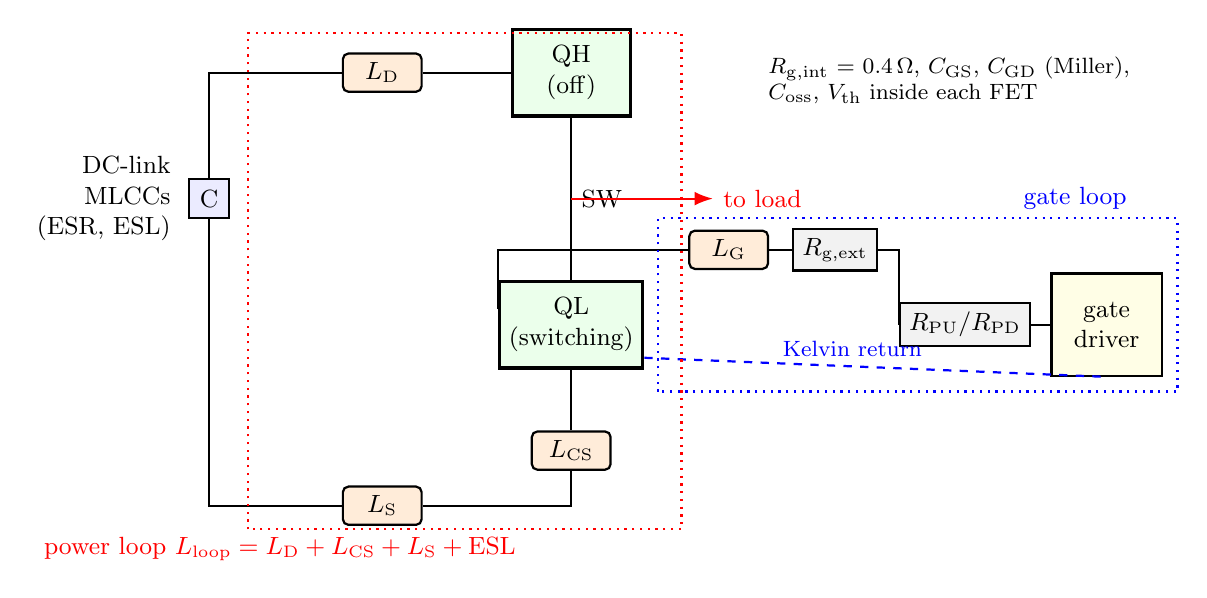
\begin{tikzpicture}[x=1cm,y=1cm,>=Latex,font=\small,
  myind/.style={draw,thick,minimum width=1.0cm,minimum height=0.32cm,rounded corners=2pt,fill=orange!15},
  myres/.style={draw,thick,minimum width=0.9cm,minimum height=0.32cm,fill=gray!10},
  mycap/.style={draw,thick,minimum width=0.5cm,minimum height=0.5cm,fill=blue!8},
  myfet/.style={draw,very thick,minimum width=1.5cm,minimum height=1.1cm,fill=green!8,align=center}]
% power loop
\node[mycap] (C) at (0,2.6) {C};
\node[left=0.1 of C,align=right] {DC-link\\ MLCCs\\ (ESR, ESL)};
\node[myind] (Lp1) at (2.2,4.2) {$L_\mathrm{D}$};
\node[myfet] (QH) at (4.6,4.2) {QH\\(off)};
\node[myfet] (QL) at (4.6,1.0) {QL\\(switching)};
\node[myind] (Lcs) at (4.6,-0.6) {$L_\mathrm{CS}$};
\node[myind] (Lp2) at (2.2,-1.3) {$L_\mathrm{S}$};
\draw[thick] (C.north) |- (Lp1.west); \draw[thick] (Lp1.east) -- (QH.west|-Lp1);
\draw[thick] (QH.south) -- node[right]{SW} (QL.north);
\draw[thick] (QL.south) -- (Lcs.north); \draw[thick] (Lcs.south) |- (Lp2.east); \draw[thick] (Lp2.west) -| (C.south);
\draw[thick,->,red] (4.6,2.6) -- (6.4,2.6) node[right,text=red]{to load};
% gate loop
\node[myres] (Rdrv) at (9.6,1.0) {$R_\mathrm{PU}/R_\mathrm{PD}$};
\node[myres] (Rg) at (7.95,1.95) {$R_\mathrm{g,ext}$};
\node[myind] (Lg) at (6.6,1.95) {$L_\mathrm{G}$};
\node[draw,thick,minimum width=1.4cm,minimum height=1.3cm,fill=yellow!10,align=center] (Drv) at (11.4,1.0) {gate\\driver};
\draw[thick] (Drv.west) -- (Rdrv.east); \draw[thick] (Rdrv.west) |- (Rg.east); \draw[thick] (Rg.west) -- (Lg.east); \draw[thick] (Lg.west) -| ($(QL.north west)!0.5!(QL.south west)+(0,0.2)$);
\draw[thick,dashed,blue] ($(QL.south east)+(0,0.15)$) -- ($(Drv.south)+(0,0.0)$) node[above,text=blue,pos=0.45,font=\footnotesize]{Kelvin return};
\node[align=left,font=\footnotesize] at (9.4,4.1) {$R_\mathrm{g,int}$ = 0.4\,$\Omega$, $C_\mathrm{GS}$, $C_\mathrm{GD}$ (Miller),\\$C_\mathrm{oss}$, $V_\mathrm{th}$ inside each FET};
\draw[dotted,thick,red] (0.5,-1.6) rectangle (6.0,4.7); \node[red] at (0.9,-1.85) {power loop $L_\mathrm{loop}=L_\mathrm{D}+L_\mathrm{CS}+L_\mathrm{S}+\mathrm{ESL}$};
\draw[dotted,thick,blue] (5.7,0.15) rectangle (12.3,2.35); \node[blue] at (11.0,2.6) {gate loop};
\end{tikzpicture}
\caption{Parasitics of one switch position (shown for QL switching, QH off). $L_\mathrm{CS}$ is the part of the source path shared by the power loop and the gate loop. With a Kelvin return it is only the few pH inside the package and pad; without one it is the whole source inductance. The same structure applies to QH, whose gate loop is referenced to the switch node.}
\end{figure}

\section{Summary map}
\renewcommand{\arraystretch}{1.25}
\begin{longtable}{@{}L{2.6cm}L{3.1cm}L{4.4cm}L{3.3cm}L{3.0cm}@{}}
\toprule
Parameter & Affects & Mechanism / equation & Constraint & This design \\\midrule\endhead
Power-loop inductance $L_\mathrm{loop}$ & $V_\mathrm{DS}$ overshoot, ringing, EMI, $E_\mathrm{off}$ & $\Delta V = L_\mathrm{loop}\,di/dt$; $f_r = 1/(2\pi\sqrt{L_\mathrm{loop} C_\mathrm{oss}})$ & $\Delta V\leq15$\,V design (90\,V), $\leq25$\,V absolute (100\,V) & 0.37\,nH per cell (Q3D, excl.\ package); peak 83--85\,V at 160\,A \\
Common-source inductance $L_\mathrm{CS}$ & Turn-on speed, $E_\mathrm{on}$, gate bump, current sharing & $v = L_\mathrm{CS}\,di_D/dt$ subtracts from (or adds to) the gate drive & $L_\mathrm{CS}\,di/dt\leq0.2$\,V $\Rightarrow$ $L_\mathrm{CS}\lesssim10$\,pH: Kelvin return required & Kelvin pickup at each source pad \\
Gate-loop inductance $L_\mathrm{G}$ & $V_\mathrm{GS}$ overshoot/undershoot, gate delay, gate bump, sharing (if unequal) & Series RLC with $C_\mathrm{iss}$: $\zeta=\tfrac{R_\mathrm{tot}}{2}\sqrt{C_\mathrm{iss}/L_\mathrm{G}}$; delay $\approx L_\mathrm{G}/R_\mathrm{tot}$ & $\zeta\geq0.5$ on turn-on; $V_\mathrm{GS}\in[-4,+6]$\,V abs; $\Delta L_\mathrm{G}\lesssim1$\,nH between parallel FETs & 1.70\,nH per FET (2.21\,nH both driven), equal star branches \\
R$_\mathrm{g,on}$ (+ driver pull-up + R$_\mathrm{g,int}$) & di/dt, dv/dt at turn-on, $E_\mathrm{on}$, overshoot, bump on the complementary FET & $I_\mathrm{G}=(V_\mathrm{drv}-V_\mathrm{pl})/R_\mathrm{on,tot}$; $t_\mathrm{vf}\approx Q_\mathrm{GD}/I_\mathrm{G}$ & Overshoot and bump limits set the minimum; $E_\mathrm{on}$ / efficiency set the maximum & 2\,$\Omega$ (total 3.0\,$\Omega$ with LT8418) \\
R$_\mathrm{g,off}$ (+ pull-down + R$_\mathrm{g,int}$) & Hold-off against Miller turn-on, turn-off speed, gate undershoot & Bump $\approx C_\mathrm{GD}\,dv/dt\cdot R_\mathrm{off,tot}$ (+ $L_\mathrm{G}$ effect) & Bump $\leq1$\,V; $V_\mathrm{GS,min}\geq-4$\,V & 0\,$\Omega$ (total 0.6\,$\Omega$); bump 0.98\,V, $V_\mathrm{GS,min}=-1.3$\,V \\
Driver source current / $R_\mathrm{PU}$ & Achievable turn-on speed, $E_\mathrm{on}$ & $I_\mathrm{G,pl}=(V_\mathrm{drv}-V_\mathrm{pl})/(R_\mathrm{PU}+\dots)$ & $\geq$\,2--4\,A peak for 2 FETs at 120\,A & LT8418 4\,A/0.6\,$\Omega$; 2EDL5014AA 4\,A/0.7\,$\Omega$ \\
Driver sink current / $R_\mathrm{PD}$ & Hold-off, bump, turn-off & as R$_\mathrm{g,off}$ & $R_\mathrm{PD}\lesssim0.5$\,$\Omega$, $\geq$\,4\,A & 0.2\,$\Omega$ (LT8418); 0.47 / 0.37\,$\Omega$ with Miller clamp (2EDL5014AA) \\
Driver voltage rating, bootstrap clamp & Survival, $V_\mathrm{GS,HS}$ & $V_\mathrm{HB}=V_\mathrm{bus}+\Delta V+V_\mathrm{boot}$; $V_\mathrm{HB-HS}=V_\mathrm{DD}+|V_\mathrm{SD}|$ without clamp & $\geq95$\,V (prefer $\geq110$\,V); $V_\mathrm{HB-HS}\leq6$\,V (GaN gate) & 100\,V (LT8418), 120\,V (2EDL5014AA), both clamp \\
Driver delay matching, CMTI & Dead time, shoot-through, false triggering & -- & matching $\ll t_\mathrm{dead}$; dv/dt rating $\geq$ 2$\times$ max dv/dt & 1--3.5\,ns; 100\,V/ns rating vs 12--32\,V/ns \\
$V_\mathrm{th}$ spread & Dynamic sharing ($E_\mathrm{on}$/$E_\mathrm{off}$ split) & Earlier/later conduction & Match devices if needed & 0.3\,V spread gives 7\,\% and a 2:1 $E_\mathrm{off}$ split \\
$Q_\mathrm{GD}$, $C_\mathrm{rss}$ & Turn-on time, gate bump & $t_\mathrm{vf}\approx Q_\mathrm{GD}/I_\mathrm{G}$; $i=C_\mathrm{GD}\,dv/dt$ & -- & 3.8\,nC, 13\,pF at 50\,V \\
$Q_\mathrm{oss}$ & $E_\mathrm{on}$ floor & $E\approx Q_\mathrm{oss}V$ even at zero current & -- & 113\,nC, 2.9\,\textmu J per FET at 75\,V \\
Dead time $t_\mathrm{dt}$ & Reverse-conduction loss, shoot-through margin & $P=2f_\mathrm{sw}t_\mathrm{dt}\overline{V_\mathrm{SD}|i|}$ & $t_\mathrm{dt}\geq$ delay mismatch + switching time & 10\,ns, 0.2\,W at 50\,kHz \\
DC-link $C$, ESR, ESL & Bus ripple, capacitor heating, part of $L_\mathrm{loop}$, resonances & $\Delta V_\mathrm{pp}\approx\hat I/(4f C)$; ESL/$N$ in the loop & $\pm2$\,\% ripple; $I_\mathrm{rms}$ per part within rating & 77\,\uF{} eff.; 0.9--2.1\,A per part; resonance 1.8/3.3\,MHz \\
L1--L2 dielectric $h$ & $L_\mathrm{loop}$ & $L\approx\mu_0 h\,l/w$ & thin (0.1\,mm) & 0.075/0.1/0.2\,mm: 0.30/0.34/0.50\,nH \\
Copper weight, terminal placement & PCB conduction loss & $P=I^2R$ with Q3D DC R & fits the loss budget & 1\,oz 4.7\,W, 2\,oz 3.3\,W \\
Layout symmetry & Static and dynamic sharing & mismatch in $L_\mathrm{G}$, $L_\mathrm{CS}$, $L_\mathrm{D}$ & mirrored geometry & L/R difference $<0.1$\,\% \\
\bottomrule
\end{longtable}

\section{Power-loop inductance: drain-source overshoot}
\textbf{Mechanism.} When a device turns off, or the complementary device's current commutates, the current in the loop formed by the DC-link capacitors and the two switches changes at $di/dt$. The loop inductance adds $L_\mathrm{loop}\,di/dt$ on top of the bus voltage across the device that is turning off, then rings with the output capacitance:
\begin{equation}
V_\mathrm{DS,pk}\approx V_\mathrm{bus}+L_\mathrm{loop}\frac{di}{dt},\qquad f_r=\frac{1}{2\pi\sqrt{L_\mathrm{loop}C_\mathrm{oss}}}.
\end{equation}
\textbf{Constraint.} Device rating 100\,V at 75\,V gives an absolute budget of 25\,V. The design budget used here is 15\,V (90\,V), which leaves margin for bus tolerance and model error:
\begin{equation}
L_\mathrm{loop}\leq\frac{\Delta V_\mathrm{max}}{di/dt}=\frac{15\,\mathrm{V}}{40\,\mathrm{A/ns}}\approx0.37\,\mathrm{nH}\quad\text{(per cell loop, 40\,A/ns per cell)}.
\end{equation}
\textbf{This design.} Q3D: 0.374\,nH per cell including MLCC ESL (package inductance not included); each cell commutates half of the load current. LTspice at 160\,A: 83\,V (QH, at QL turn-on) and 85\,V (QL turn-off); ringing near 330\,MHz, consistent with the 0.374\,nH cell loop and the $C_\mathrm{oss}$ of one FET at 75\,V ($\approx$\,0.6\,nF). Also affected: $E_\mathrm{off}$ (energy in the ringing), EMI, and the turn-on rate that can be allowed.

\textbf{Levers.} Thin L1--L2 dielectric (0.1\,mm), commutation capacitors right at the high-side drain, many return vias, wide short copper, low-ESL capacitors in parallel. If overshoot is still too high: increase R$_\mathrm{g,on}$, since di/dt at turn-on is gate-controlled. At high current, turn-off di/dt is load-driven and hardly controllable.

\section{Common-source inductance: slower switching, gate bump, sharing}
\textbf{Mechanism.} Inductance shared by the drain-source current and the gate return ($L_\mathrm{CS}$) induces $L_\mathrm{CS}\,di_D/dt$ in the gate loop (AN020):
\begin{equation}
I_\mathrm{G}=\frac{V_\mathrm{drv}-V_\mathrm{GS}-L_\mathrm{CS}\,di_D/dt}{R_\mathrm{tot}}.
\end{equation}
At turn-on it opposes the drive: slower di/dt, higher $E_\mathrm{on}$ (negative feedback). For the off device, the di/dt of its own reverse current during the complementary commutation induces a gate voltage of either sign, which adds to the Miller bump. Between paralleled devices, unequal $L_\mathrm{CS}$ gives unequal effective drive, which is the worst current-sharing mechanism.

\textbf{Constraint.} Keep $L_\mathrm{CS}\,di/dt$ well below the threshold margin. With 20\,A/ns per device and $\leq$0.2\,V allowed, $L_\mathrm{CS}\lesssim10$\,pH. Only a Kelvin source return (gate return taken at the source pad nearest the gate) achieves this.

\textbf{Evidence.} Sharing study (two EPC2361, LTspice): symmetric $L_\mathrm{CS}$ without Kelvin raised $E_\mathrm{on}$ by 47\,\% and lowered overshoot; $L_\mathrm{CS}$ imbalance of 0.2\,nH gave 29\,\% dynamic current imbalance (144 vs 79\,A) and a 2.8:1 $E_\mathrm{on}$ split. With a source shunt in the power path, the shunt sits outside the gate loop only if the Kelvin pickup is on the device side.

\section{Gate-loop inductance: gate ringing, delay, and its role in the bump}
\textbf{Mechanism.} $L_\mathrm{G}$, $R_\mathrm{tot}$ and $C_\mathrm{iss}$ form a series RLC:
\begin{equation}
f_0=\frac{1}{2\pi\sqrt{L_\mathrm{G}C_\mathrm{iss}}},\qquad \zeta=\frac{R_\mathrm{tot}}{2}\sqrt{\frac{C_\mathrm{iss}}{L_\mathrm{G}}},\qquad \tau\approx\frac{L_\mathrm{G}}{R_\mathrm{tot}}.
\end{equation}
Low damping gives $V_\mathrm{GS}$ overshoot at turn-on (limit +6\,V absolute, 5\,V recommended) and undershoot at turn-off (limit $-4$\,V). $L_\mathrm{G}$ also delays the gate and stops the driver from removing Miller charge quickly, which enlarges the gate bump.

\textbf{This design.} $L_\mathrm{G}$ = 1.7\,nH, $C_\mathrm{iss}$ = 3.6\,nF: $f_0\approx64$\,MHz.
Turn-on path $R_\mathrm{tot}=0.6+2+0.4=3.0\,\Omega$ gives $\zeta\approx2.2$ (no overshoot).
Turn-off path $0.2+0+0.4=0.6\,\Omega$ gives $\zeta\approx0.44$; the result is the $-1.3$\,V undershoot seen in LTspice, inside the $-4$\,V limit.
Constraint for well-damped turn-on: $\zeta\geq0.5$, i.e.\ $R_\mathrm{on,tot}\geq\sqrt{L_\mathrm{G}/C_\mathrm{iss}}\approx0.7\,\Omega$.

\textbf{Paralleling.} Unequal $L_\mathrm{G}$ means unequal delay $\Delta t\approx\Delta L_\mathrm{G}/R_\mathrm{tot}$. When $\Delta t$ approaches the voltage transition (about 4\,ns), one device carries the whole switching event: 2 vs 8\,nH gave about 2\,ns delay, a 19\,\% current imbalance and a 4:1 $E_\mathrm{on}$ split. A practical rule is $\Delta t\leq t_\mathrm{vf}/10$, so $\Delta L_\mathrm{G}\lesssim0.1\cdot4\,\mathrm{ns}\cdot3\,\Omega\approx1$\,nH, which in practice means equal star branches (here: driver on the symmetry line, $<0.1$\,\% mismatch).

\section{Gate resistances and gate-driver strength}
The resistance seen by each gate is the sum of the driver output resistance, the external resistor and the internal gate resistance:
\begin{equation}
R_\mathrm{on,tot}=R_\mathrm{PU}+R_\mathrm{g,on}+R_\mathrm{g,int},\qquad R_\mathrm{off,tot}=R_\mathrm{PD}+R_\mathrm{g,off}+R_\mathrm{g,int}.
\end{equation}
When one driver output feeds two FETs, $R_\mathrm{PU}$ and $R_\mathrm{PD}$ are shared, so each gate sees roughly twice their value during simultaneous switching.

\textbf{Turn-on (R$_\mathrm{g,on}$, driver source).} The plateau current $I_\mathrm{G}=(V_\mathrm{drv}-V_\mathrm{pl})/R_\mathrm{on,tot}$ sets the current rise time $t_\mathrm{ri}\approx(Q_\mathrm{GS}-Q_\mathrm{G(th)})/I_\mathrm{G}$ and the voltage fall time $t_\mathrm{vf}\approx Q_\mathrm{GD}/I_\mathrm{G}$, therefore di/dt (overshoot), dv/dt (bump on the complementary FET, EMI) and
\begin{equation}
E_\mathrm{on}\approx\tfrac12 V I\,(t_\mathrm{ri}+t_\mathrm{vf})+Q_\mathrm{oss}V.
\end{equation}
Sweep at 160\,A (LT8418, $R_\mathrm{g,off}$ = 0):
\begin{center}\small
\begin{tabular}{@{}lccccc@{}}\toprule
R$_\mathrm{g,on}$ [$\Omega$] & 0.5 & 1 & 1.5 & 2 & 4 \\\midrule
QH overshoot peak [V] & 112 & 95 & 86.5 & 83.1 & 76.8 \\
$E_\mathrm{on}$ [\textmu J] & 27.7 & 35.0 & 41.5 & 47.4 & 68.0 \\
Bump on QH [V] & 1.12 & 1.07 & 1.02 & 0.98 & 0.88 \\
\bottomrule\end{tabular}\end{center}
The lower bound of R$_\mathrm{g,on}$ is set by overshoot and bump, the upper bound by $E_\mathrm{on}$ and efficiency (or a dv/dt requirement: EPC9186 motor drive uses 10\,$\Omega$/0.47\,$\Omega$ for about 6\,V/ns; the EPC2361 datasheet board EPC90156 uses 1\,$\Omega$/0\,$\Omega$).

\textbf{Turn-off (R$_\mathrm{g,off}$, driver sink).} At high current the GaN turn-off is load-driven: once the channel closes, the load current charges $C_\mathrm{oss}$, so $E_\mathrm{off}$ is small (7--8\,\textmu J) and hardly depends on R$_\mathrm{g,off}$ (8.4 to 14.4\,\textmu J for 0 to 1\,$\Omega$ at 160\,A). Its main job is hold-off: the off-state gate must stay below threshold while the complementary device switches. A static estimate of the Miller-induced gate voltage is
\begin{equation}
V_\mathrm{bump}\approx C_\mathrm{GD}\frac{dv}{dt}R_\mathrm{off,tot}\quad(\text{lower bound}),\qquad V_\mathrm{bump}\lesssim\frac{Q_\mathrm{GD}}{C_\mathrm{iss}}\approx1\,\mathrm{V}\quad(\text{if the gate loop cannot respond}).
\end{equation}
With $L_\mathrm{G}$ = 1.7\,nH the real value (0.98\,V) is close to the upper estimate, which is why a low R$_\mathrm{g,off}$, a strong pull-down (or an active Miller clamp) and a short gate loop all matter. Constraint: bump $\leq$1\,V against $V_\mathrm{th}$ = 0.8\,V min / 1.1\,V typ (lower when hot); verify on hardware.

\textbf{Driver requirements derived from this design.}
\begin{itemize}\itemsep0pt
\item Voltage: $V_\mathrm{HB}\geq V_\mathrm{bus}+\Delta V+V_\mathrm{boot}\approx95$\,V; prefer $\geq$110\,V.
\item Bootstrap clamp: during dead time the switch node is $V_\mathrm{SD}\approx2$--3\,V below ground, so an unclamped bootstrap charges to 7--8\,V, above the 6\,V GaN gate limit. A clamp or smart bootstrap switch is required (LT8418, 2EDL501xAA).
\item Source $\geq$2--4\,A (about 0.6--0.7\,$\Omega$), sink $\geq$4\,A ($\leq$0.5\,$\Omega$), split outputs for independent R$_\mathrm{g,on}$/R$_\mathrm{g,off}$; 1.5\,A-source drivers (LMG1210, 2EDL5012AA) were too slow at 120\,A.
\item dv/dt immunity $\geq$100\,V/ns (we see 12--32\,V/ns); HO/LO delay matching of a few ns; UVLO compatible with 5\,V gates.
\item Bootstrap recharge: switch resistance and minimum low-side on-time limit the high-side gate voltage at high modulation index (2EDL5014AA: 6--9\,$\Omega$ gives about 0.8--1.2\,V droop at 0.5\,\textmu s on-time).
\end{itemize}

\section{Device parameters and spread}
\begin{itemize}\itemsep0pt
\item $R_\mathrm{DS(on)}$ (0.75/1.0\,m$\Omega$, $\times$1.48 at 100\,$^\circ$C): conduction loss $I^2R/2$ = 5.6\,W per leg; sets static sharing (its positive temperature coefficient self-balances).
\item $V_\mathrm{th}$ spread: dynamic sharing. 0.3\,V gives 7\,\% turn-on imbalance and a 2:1 turn-off energy split; the low-threshold device turns off last and briefly carries 80\,A. Not fixable by layout.
\item $Q_\mathrm{GD}$ / $C_\mathrm{rss}$: switching speed and Miller bump. $Q_\mathrm{oss}$: an $E_\mathrm{on}$ floor of about 2\,$\times$\,113\,nC\,$\times$\,75\,V even at zero current.
\item $V_\mathrm{SD}$ in reverse conduction (about 2--2.5\,V): dead-time loss and bootstrap overcharge.
\end{itemize}

\section{Dead time}
Lower bound: driver delay mismatch (1--3.5\,ns) plus the device switching time (about 4--6\,ns), otherwise shoot-through. Upper bound: reverse-conduction loss $2f_\mathrm{sw}t_\mathrm{dt}\overline{V_\mathrm{SD}|i|}$ (0.2\,W at 10\,ns and 50\,kHz) and the bootstrap behaviour. 10--20\,ns is a reasonable starting range; tune on hardware.

\section{DC-link capacitors and stack-up}
\begin{itemize}\itemsep0pt
\item Capacitance sets the bus ripple: $\Delta V_\mathrm{pp}\approx\hat I/(4f_\mathrm{sw}C)$ per isolated leg; three legs on one bank need the same total, so a third per leg (78\,\uF{} effective per leg for $\pm$2\,\% at 50\,kHz).
\item ESL of the commutation capacitors is part of $L_\mathrm{loop}$ (6\,$\times$\,0.48\,nH in parallel adds about 0.08\,nH per cell); place them at the high-side drain.
\item ESR sets heating: 0.9--2.1\,A$_\mathrm{rms}$ per part, about 0.2\,W total; check against the manufacturer ripple rating.
\item Small local banks plus large bulk rows resonate through the copper inductance (1.8 and 3.3\,MHz here); damp with a higher-ESR part if it shows up in ringing or EMI.
\item L1--L2 dielectric: $L\propto h$ (0.075/0.1/0.2\,mm gives 0.30/0.34/0.50\,nH). Copper weight and DC-terminal placement set the PCB conduction loss (1\,oz 4.7\,W, 2\,oz 3.3\,W); heavy copper must not force a thicker L1--L2 prepreg.
\end{itemize}

\section{Design checklist}
\begin{center}\small
\begin{tabular}{@{}L{6.2cm}L{4.6cm}L{3.6cm}@{}}\toprule
Check & Limit & Status \\\midrule
$V_\mathrm{DS}$ peak at 1.13\,$\times$\,max current & $\leq$90\,V design, $\leq$100\,V absolute & 83--85\,V \\
$V_\mathrm{GS}$ peak / minimum & $\leq$6\,V / $\geq-4$\,V & 5\,V / $-1.3$\,V \\
Off-state gate bump & $\leq$1\,V (vs $V_\mathrm{th,min}$ = 0.8\,V) & 0.98\,V, verify \\
$L_\mathrm{CS}$ & Kelvin return, $\lesssim$10\,pH & Kelvin at each source pad \\
Gate-branch mismatch $\Delta L_\mathrm{G}$ & $\lesssim$1\,nH & $<$0.1\,\% \\
Gate damping at turn-on & $\zeta\geq0.5$ & $\zeta\approx2.2$ \\
Driver $V_\mathrm{HB}$ rating & $\geq$95\,V (prefer 110\,V) & 100\,V / 120\,V \\
Bootstrap $V_\mathrm{HB-HS}$ & $\leq$6\,V with negative switch node & clamped \\
Switch-node dv/dt vs driver rating & $\leq$50\,\% of rating & 12--32 of 100\,V/ns \\
DC-link ripple & $\pm$2\,\% & meets on shared bus \\
Loss & $\leq$13.3\,W per leg (99.5\,\%) & 11.1\,W \\
\bottomrule\end{tabular}\end{center}

\textbf{Sources.} EPC2361 datasheet rev.~2.4; EPC AN020 (paralleling, common-source inductance), AN023 (measurement); EPC90156, EPC90135, EPC9186 board data; LT8418 and 2EDL501xAA-U2D datasheets; Q3D and LTspice results in \texttt{simulation/} (bb\_q3d, bb\_spice, sharing, q3d).
\end{document}
